% Options for packages loaded elsewhere
\PassOptionsToPackage{unicode}{hyperref}
\PassOptionsToPackage{hyphens}{url}
\PassOptionsToPackage{dvipsnames,svgnames,x11names}{xcolor}
%
\documentclass[
  letterpaper,
  DIV=11,
  numbers=noendperiod]{scrartcl}

\usepackage{amsmath,amssymb}
\usepackage{iftex}
\ifPDFTeX
  \usepackage[T1]{fontenc}
  \usepackage[utf8]{inputenc}
  \usepackage{textcomp} % provide euro and other symbols
\else % if luatex or xetex
  \usepackage{unicode-math}
  \defaultfontfeatures{Scale=MatchLowercase}
  \defaultfontfeatures[\rmfamily]{Ligatures=TeX,Scale=1}
\fi
\usepackage{lmodern}
\ifPDFTeX\else  
    % xetex/luatex font selection
\fi
% Use upquote if available, for straight quotes in verbatim environments
\IfFileExists{upquote.sty}{\usepackage{upquote}}{}
\IfFileExists{microtype.sty}{% use microtype if available
  \usepackage[]{microtype}
  \UseMicrotypeSet[protrusion]{basicmath} % disable protrusion for tt fonts
}{}
\makeatletter
\@ifundefined{KOMAClassName}{% if non-KOMA class
  \IfFileExists{parskip.sty}{%
    \usepackage{parskip}
  }{% else
    \setlength{\parindent}{0pt}
    \setlength{\parskip}{6pt plus 2pt minus 1pt}}
}{% if KOMA class
  \KOMAoptions{parskip=half}}
\makeatother
\usepackage{xcolor}
\setlength{\emergencystretch}{3em} % prevent overfull lines
\setcounter{secnumdepth}{-\maxdimen} % remove section numbering
% Make \paragraph and \subparagraph free-standing
\ifx\paragraph\undefined\else
  \let\oldparagraph\paragraph
  \renewcommand{\paragraph}[1]{\oldparagraph{#1}\mbox{}}
\fi
\ifx\subparagraph\undefined\else
  \let\oldsubparagraph\subparagraph
  \renewcommand{\subparagraph}[1]{\oldsubparagraph{#1}\mbox{}}
\fi

\usepackage{color}
\usepackage{fancyvrb}
\newcommand{\VerbBar}{|}
\newcommand{\VERB}{\Verb[commandchars=\\\{\}]}
\DefineVerbatimEnvironment{Highlighting}{Verbatim}{commandchars=\\\{\}}
% Add ',fontsize=\small' for more characters per line
\usepackage{framed}
\definecolor{shadecolor}{RGB}{241,243,245}
\newenvironment{Shaded}{\begin{snugshade}}{\end{snugshade}}
\newcommand{\AlertTok}[1]{\textcolor[rgb]{0.68,0.00,0.00}{#1}}
\newcommand{\AnnotationTok}[1]{\textcolor[rgb]{0.37,0.37,0.37}{#1}}
\newcommand{\AttributeTok}[1]{\textcolor[rgb]{0.40,0.45,0.13}{#1}}
\newcommand{\BaseNTok}[1]{\textcolor[rgb]{0.68,0.00,0.00}{#1}}
\newcommand{\BuiltInTok}[1]{\textcolor[rgb]{0.00,0.23,0.31}{#1}}
\newcommand{\CharTok}[1]{\textcolor[rgb]{0.13,0.47,0.30}{#1}}
\newcommand{\CommentTok}[1]{\textcolor[rgb]{0.37,0.37,0.37}{#1}}
\newcommand{\CommentVarTok}[1]{\textcolor[rgb]{0.37,0.37,0.37}{\textit{#1}}}
\newcommand{\ConstantTok}[1]{\textcolor[rgb]{0.56,0.35,0.01}{#1}}
\newcommand{\ControlFlowTok}[1]{\textcolor[rgb]{0.00,0.23,0.31}{#1}}
\newcommand{\DataTypeTok}[1]{\textcolor[rgb]{0.68,0.00,0.00}{#1}}
\newcommand{\DecValTok}[1]{\textcolor[rgb]{0.68,0.00,0.00}{#1}}
\newcommand{\DocumentationTok}[1]{\textcolor[rgb]{0.37,0.37,0.37}{\textit{#1}}}
\newcommand{\ErrorTok}[1]{\textcolor[rgb]{0.68,0.00,0.00}{#1}}
\newcommand{\ExtensionTok}[1]{\textcolor[rgb]{0.00,0.23,0.31}{#1}}
\newcommand{\FloatTok}[1]{\textcolor[rgb]{0.68,0.00,0.00}{#1}}
\newcommand{\FunctionTok}[1]{\textcolor[rgb]{0.28,0.35,0.67}{#1}}
\newcommand{\ImportTok}[1]{\textcolor[rgb]{0.00,0.46,0.62}{#1}}
\newcommand{\InformationTok}[1]{\textcolor[rgb]{0.37,0.37,0.37}{#1}}
\newcommand{\KeywordTok}[1]{\textcolor[rgb]{0.00,0.23,0.31}{#1}}
\newcommand{\NormalTok}[1]{\textcolor[rgb]{0.00,0.23,0.31}{#1}}
\newcommand{\OperatorTok}[1]{\textcolor[rgb]{0.37,0.37,0.37}{#1}}
\newcommand{\OtherTok}[1]{\textcolor[rgb]{0.00,0.23,0.31}{#1}}
\newcommand{\PreprocessorTok}[1]{\textcolor[rgb]{0.68,0.00,0.00}{#1}}
\newcommand{\RegionMarkerTok}[1]{\textcolor[rgb]{0.00,0.23,0.31}{#1}}
\newcommand{\SpecialCharTok}[1]{\textcolor[rgb]{0.37,0.37,0.37}{#1}}
\newcommand{\SpecialStringTok}[1]{\textcolor[rgb]{0.13,0.47,0.30}{#1}}
\newcommand{\StringTok}[1]{\textcolor[rgb]{0.13,0.47,0.30}{#1}}
\newcommand{\VariableTok}[1]{\textcolor[rgb]{0.07,0.07,0.07}{#1}}
\newcommand{\VerbatimStringTok}[1]{\textcolor[rgb]{0.13,0.47,0.30}{#1}}
\newcommand{\WarningTok}[1]{\textcolor[rgb]{0.37,0.37,0.37}{\textit{#1}}}

\providecommand{\tightlist}{%
  \setlength{\itemsep}{0pt}\setlength{\parskip}{0pt}}\usepackage{longtable,booktabs,array}
\usepackage{calc} % for calculating minipage widths
% Correct order of tables after \paragraph or \subparagraph
\usepackage{etoolbox}
\makeatletter
\patchcmd\longtable{\par}{\if@noskipsec\mbox{}\fi\par}{}{}
\makeatother
% Allow footnotes in longtable head/foot
\IfFileExists{footnotehyper.sty}{\usepackage{footnotehyper}}{\usepackage{footnote}}
\makesavenoteenv{longtable}
\usepackage{graphicx}
\makeatletter
\def\maxwidth{\ifdim\Gin@nat@width>\linewidth\linewidth\else\Gin@nat@width\fi}
\def\maxheight{\ifdim\Gin@nat@height>\textheight\textheight\else\Gin@nat@height\fi}
\makeatother
% Scale images if necessary, so that they will not overflow the page
% margins by default, and it is still possible to overwrite the defaults
% using explicit options in \includegraphics[width, height, ...]{}
\setkeys{Gin}{width=\maxwidth,height=\maxheight,keepaspectratio}
% Set default figure placement to htbp
\makeatletter
\def\fps@figure{htbp}
\makeatother

\KOMAoption{captions}{tableheading}
\makeatletter
\@ifpackageloaded{caption}{}{\usepackage{caption}}
\AtBeginDocument{%
\ifdefined\contentsname
  \renewcommand*\contentsname{Table of contents}
\else
  \newcommand\contentsname{Table of contents}
\fi
\ifdefined\listfigurename
  \renewcommand*\listfigurename{List of Figures}
\else
  \newcommand\listfigurename{List of Figures}
\fi
\ifdefined\listtablename
  \renewcommand*\listtablename{List of Tables}
\else
  \newcommand\listtablename{List of Tables}
\fi
\ifdefined\figurename
  \renewcommand*\figurename{Figure}
\else
  \newcommand\figurename{Figure}
\fi
\ifdefined\tablename
  \renewcommand*\tablename{Table}
\else
  \newcommand\tablename{Table}
\fi
}
\@ifpackageloaded{float}{}{\usepackage{float}}
\floatstyle{ruled}
\@ifundefined{c@chapter}{\newfloat{codelisting}{h}{lop}}{\newfloat{codelisting}{h}{lop}[chapter]}
\floatname{codelisting}{Listing}
\newcommand*\listoflistings{\listof{codelisting}{List of Listings}}
\makeatother
\makeatletter
\makeatother
\makeatletter
\@ifpackageloaded{caption}{}{\usepackage{caption}}
\@ifpackageloaded{subcaption}{}{\usepackage{subcaption}}
\makeatother
\ifLuaTeX
  \usepackage{selnolig}  % disable illegal ligatures
\fi
\usepackage{bookmark}

\IfFileExists{xurl.sty}{\usepackage{xurl}}{} % add URL line breaks if available
\urlstyle{same} % disable monospaced font for URLs
\hypersetup{
  pdftitle={PSC 103B - Lab 4 Assignment},
  colorlinks=true,
  linkcolor={blue},
  filecolor={Maroon},
  citecolor={Blue},
  urlcolor={Blue},
  pdfcreator={LaTeX via pandoc}}

\title{PSC 103B - Lab 4 Assignment}
\usepackage{etoolbox}
\makeatletter
\providecommand{\subtitle}[1]{% add subtitle to \maketitle
  \apptocmd{\@title}{\par {\large #1 \par}}{}{}
}
\makeatother
\subtitle{Answer Key}
\author{}
\date{}

\begin{document}
\maketitle

\subsection{The data}\label{the-data}

This week, we will be moving away from the NPAS dataset and using the
version of the penguins dataset that we have been using in lab. Download
this dataset from the Homework 5 assignment page on Canvas.

The variables we will be using today are:

\begin{itemize}
\tightlist
\item
  \texttt{species}: The species of the penguin (Adelie, Chinstrap, or
  Gentoo)
\item
  \texttt{sex}: The sex of the penguin (male or female)
\item
  \texttt{bill\_length\_mm}: The bill length of the penguin, measured in
  mm
\end{itemize}

\begin{Shaded}
\begin{Highlighting}[]
\NormalTok{hw\_data }\OtherTok{\textless{}{-}} \FunctionTok{read.csv}\NormalTok{(}\StringTok{"../lab/data/penguins\_103b.csv"}\NormalTok{)}
\end{Highlighting}
\end{Shaded}

\section{Question 1}\label{question-1}

Suppose we were interested in conducting a factorial ANOVA with species
and sex as our grouping variables, and bill length as the outcome.

Write out the 3 sets of null and alternative hypotheses for the
factorial ANOVA -- one for each main effect and one for the interaction.
(3 points)

\textbf{Hypotheses for Main Effect of Species}

\[
H_0: \mu_{Adelie} = \mu_{Chinstrap} = \mu_{Gentoo}\\
H_1: \text{At least one mean is not equal to the rest}
\] Where \(\mu\) represents the average bill length

\textbf{Hypotheses for Main Effect of Sex}

\[
H_0: \mu_{Female} = \mu_{Male}\\
H_1: \mu_{Female} \neq \mu_{Male}
\]

Where \(\mu\) represents the average bill length (note that our
alternative hypothesis can be so specific because we only have 2
groups).

\textbf{Hypotheses for the Interaction}

\[
H_0: \text{There is no interaction between species and sex on bill length}\\
H_1: \text{There is an interaction between species and sec on bill length}
\]

\section{Question 2}\label{question-2}

Conduct the factorial ANOVA. Show your code and output. (1 point)

\begin{Shaded}
\begin{Highlighting}[]
\NormalTok{fact\_anova }\OtherTok{\textless{}{-}} \FunctionTok{aov}\NormalTok{(bill\_length\_mm }\SpecialCharTok{\textasciitilde{}}\NormalTok{ species}\SpecialCharTok{*}\NormalTok{sex, }\AttributeTok{data =}\NormalTok{ hw\_data)}
\FunctionTok{summary}\NormalTok{(fact\_anova)}
\end{Highlighting}
\end{Shaded}

\begin{verbatim}
             Df Sum Sq Mean Sq F value Pr(>F)    
species       2   4376  2187.8 399.792 <2e-16 ***
sex           1    752   752.0 137.424 <2e-16 ***
species:sex   2     18     9.1   1.669  0.191    
Residuals   196   1073     5.5                   
---
Signif. codes:  0 '***' 0.001 '**' 0.01 '*' 0.05 '.' 0.1 ' ' 1
2 observations deleted due to missingness
\end{verbatim}

\section{Question 3}\label{question-3}

\emph{If the main effect of dose is significant}: Conduct the Tukey
Honest Significant Difference post-hoc test. Show your code.

\emph{If the main effect of dose is not significant}: State ``The main
effect of species was not significant''. (1 point)

\begin{Shaded}
\begin{Highlighting}[]
\FunctionTok{TukeyHSD}\NormalTok{(fact\_anova, }\AttributeTok{which =} \StringTok{"species"}\NormalTok{)}
\end{Highlighting}
\end{Shaded}

\begin{verbatim}
  Tukey multiple comparisons of means
    95% family-wise confidence level

Fit: aov(formula = bill_length_mm ~ species * sex, data = hw_data)

$species
                      diff       lwr        upr    p adj
Chinstrap-Adelie 10.435316  9.484314 11.3863184 0.000000
Gentoo-Adelie     9.211940  8.257422 10.1664584 0.000000
Gentoo-Chinstrap -1.223376 -2.174378 -0.2723734 0.007592
\end{verbatim}

\section{Question 4}\label{question-4}

If you conducted the Tukey HSD test in the previous question: Which
groups were significantly different from each other? What was the
difference (e.g., which group had the larger/smaller bill length)? (1
point)

\textcolor[RGB]{178,34,34}{Adelie penguins had significantly smaller
bill lengths than both Chinstrap and Gentoo penguins, and Gentoo
penguins had significantly smaller bill lengths than Chinstrap
penguins.}

\section{Question 5}\label{question-5}

\emph{If the main effect of sex is significant}: Calculate the means for
each group. Show your code and output.

\emph{If the main effect of sex is not significant}: State ``The main
effect of sex was not significant''. (1 point)

\textcolor[RGB]{178,34,34}{The mean bill length for female penguins was
42.61 mm, whereas the mean bill length for male penguins was 47.47 mm.}

\begin{Shaded}
\begin{Highlighting}[]
\FunctionTok{tapply}\NormalTok{(hw\_data}\SpecialCharTok{$}\NormalTok{bill\_length\_mm, hw\_data}\SpecialCharTok{$}\NormalTok{sex, mean)}
\end{Highlighting}
\end{Shaded}

\begin{verbatim}
  female     male 
42.60865 47.46939 
\end{verbatim}

\section{Question 6}\label{question-6}

\emph{If you calculated the means in the previous question}: Which group
(males or females) had the longer bill length? (1 point)

\section{Question 7}\label{question-7}

Was the interaction significant? What does this tell us (e.g., does the
main effect of species depend on sex)? (1 point)

\textcolor[RGB]{178,34,34}{The interaction was not significant (p =
.19), which means that the main effect of sex does not depend on species
(or, that the main effect of species does not depend on the penguin's
sex).}

\section{Question 8}\label{question-8}

\begin{Shaded}
\begin{Highlighting}[]
\FunctionTok{interaction.plot}\NormalTok{(hw\_data}\SpecialCharTok{$}\NormalTok{species,}
\NormalTok{                 hw\_data}\SpecialCharTok{$}\NormalTok{sex,}
\NormalTok{                 hw\_data}\SpecialCharTok{$}\NormalTok{bill\_length\_mm,}
                 \AttributeTok{type =} \StringTok{"l"}\NormalTok{,}
                 \AttributeTok{xlab =} \StringTok{"Species"}\NormalTok{,}
                 \AttributeTok{ylab =} \StringTok{"Mean Bill Length"}\NormalTok{,}
                 \AttributeTok{trace.label =} \StringTok{"Sex"}\NormalTok{)}
\end{Highlighting}
\end{Shaded}

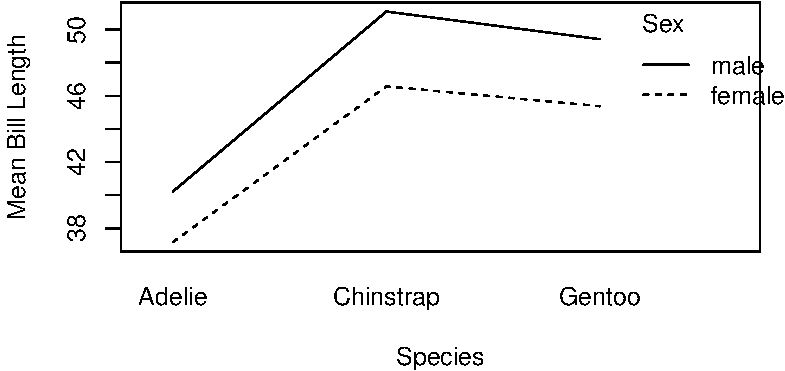
\includegraphics{103bA5_files/figure-pdf/unnamed-chunk-5-1.pdf}



\end{document}
